\documentclass[11pt]{article}
\title{\textbf{Meccano fox-surd frame}}
\author{https://github.com/heptagons/meccano/frames/fox-surd}
\date{}

\usepackage{../../meccano}
\usepackage{tikz}
\usetikzlibrary{calc}

\begin{document}

\maketitle
\begin{abstract}
Meccano\meccanoref fox-surd frame is a generalization of fox-frame\footnote{
\href{https://github.com/heptagons/meccano/blob/main/frames/fox/fox.pdf}{Meccano fox frame }}
where two of the original five strips are no longer integers but surds which must be solved
using several more strips.
\end{abstract}

\section{Pentagons fox-surd}

\begin{figure}[H]
\centering
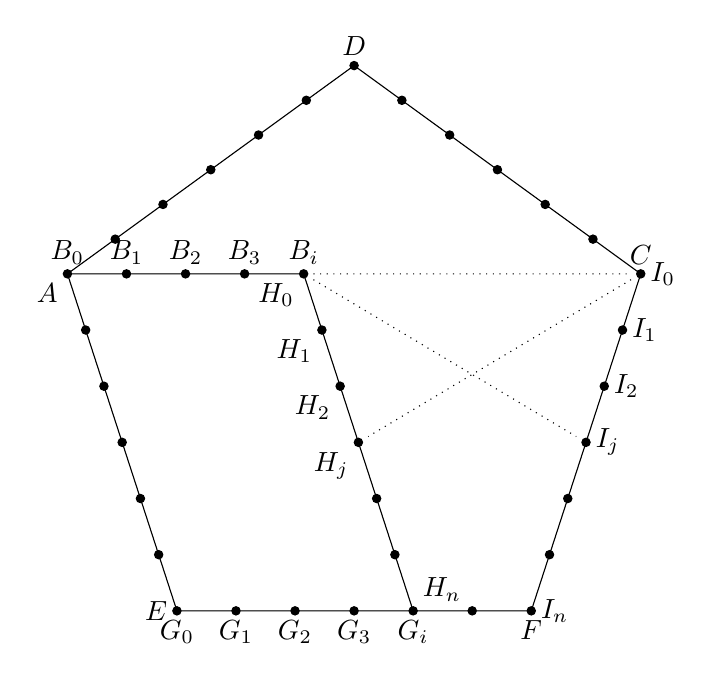
\begin{tikzpicture}
\begin{scope}[scale=0.75]
\begin{scope}
\draw[fill=black] (0,0) circle(2pt) node[above]{$B_0$}
-- ++(1,0) circle(2pt) node[above]{$B_1$}
-- ++(1,0) circle(2pt) node[above]{$B_2$}
-- ++(1,0) circle(2pt) node[above]{$B_3$}
-- ++(1,0) circle(2pt) node[above]{$B_i$} node[below left]{$H_0$} node(bi){}
-- ++(-72:1) circle(2pt) node[below left]{$H_1$}
-- ++(-72:1) circle(2pt) node[below left]{$H_2$}
-- ++(-72:1) circle(2pt) node[below left]{$H_j$} node(hj){}
-- ++(-72:1) circle(2pt)
-- ++(-72:1) circle(2pt)
-- ++(-72:1) circle(2pt) node[above right]{$H_n$} node[below]{$G_i$}
-- ++(-1,0) circle(2pt) node[below]{$G_3$}
-- ++(-1,0) circle(2pt) node[below]{$G_2$}
-- ++(-1,0) circle(2pt) node[below]{$G_1$}
-- ++(-1,0) circle(2pt) node[below]{$G_0$} node[left]{$E$}
-- ++(108:1) circle(2pt)
-- ++(108:1) circle(2pt)
-- ++(108:1) circle(2pt)
-- ++(108:1) circle(2pt)
-- ++(108:1) circle(2pt)
-- ++(108:1);
\draw[fill=black] (0,0) node[below left]{$A$}
-- ++(36:1) circle(2pt)
-- ++(36:1) circle(2pt)
-- ++(36:1) circle(2pt)
-- ++(36:1) circle(2pt)
-- ++(36:1) circle(2pt)
-- ++(36:1) circle(2pt) node[above]{$D$}
-- ++(-36:1) circle(2pt)
-- ++(-36:1) circle(2pt)
-- ++(-36:1) circle(2pt)
-- ++(-36:1) circle(2pt)
-- ++(-36:1) circle(2pt)
-- ++(-36:1) circle(2pt) node[above]{$C$} node[right]{$I_0$} node(i0){}
-- ++(-108:1) circle(2pt) node[right]{$I_1$}
-- ++(-108:1) circle(2pt) node[right]{$I_2$}
-- ++(-108:1) circle(2pt) node[right]{$I_j$} node(ij){}
-- ++(-108:1) circle(2pt)
-- ++(-108:1) circle(2pt)
-- ++(-108:1) circle(2pt) node[below]{$F$} node[right]{$I_n$}
-- ++(-1,0) circle(2pt)
-- ++(-1,0);

\draw[dotted] (bi) -- (ij) (i0) -- (hj) (bi) -- (i0);

\end{scope}
\end{scope}
\end{tikzpicture}
\caption{Pentagon of size $n$ where each segment separated by circles represents a unit.
We have a surd frame formed by the six points: $B_i$, $I_0$, $H_j$, $I_j$, $H_n$ and $I_n$.
By iterating the values $i,j = 0,...,n$ we'll get diverse frames.
}

\label{fig:pentagon}
\end{figure}

From figure \ref{fig:pentagon} the fox-surd frame has three real strips of integer size:
\begin{itemize}
    \item $\overline{B_iG_i}$ of size $n$.
    \item $\overline{G_iI_n}$ of size $n-i$, where $i = 0,...,n$.
    \item $\overline{I_nI_0}$ of size $n$.
\end{itemize}
The other two strips are generic in the sense the sizes can be surds:
\begin{itemize}
	\item $\overline{B_iI_j}$ of size $f(n,i,j)$, where $i,j = 0,...,n$.
	\item $\overline{I_0H_j}$ of equal size of $\overline{B_iI_j}$.
\end{itemize}

From the regular pentagon we know the main diagonal $\overline{AC}$ equals
$\frac{1+\sqrt{5}}{4}n$ where $n$ is the pentagon side size. We can calculate different
segments of the main diagonal iterating $i = 0,...,n$:
\begin{align}
B_0 &\equiv A \nonumber\\
\overline{B_0C} &= \frac{1+\sqrt{5}}{4}n \\
\overline{B_iC} &= \frac{1+\sqrt{5}}{4}n - i \nonumber\\
 &= \frac{n-4i}{4} + \frac{\sqrt{5}}{4}, \quad i = 0, ..., n \label{eq:B_iC}
\end{align}

From the regular pentagon we know the angle ${CB_iH_i}$ equals $2\pi / 5$ so we have:
\begin{align}
\theta &\equiv \angle{CB_iH_i} \\
\cos\theta &= \cos\frac{2\pi}{5} = \frac{\sqrt{5}-1}{4} \label{eq:cosine}
\end{align}

\subsection{Surds strips}

Using the law of cosines we can calculate one of the frame surds $s_ij \equiv \overline{B_iH_j}$.
We notice the value of $\overline{B_iH_i}$ equals $i$, and we'll use the values of $\overline{B_iC}$ from equation \ref{eq:B_iC}, and the cosine value from equation \ref{eq:cosine} to get:
\begin{align}
s_i^2 &\equiv \overline{CH_i}^2 \\
 &= \overline{B_iH_i}^2 + \overline{B_iC}^2
 - 2\overline{B_iH_i}\times\overline{B_iC}\cos\theta  \nonumber\\
  &= i^2 + \left(\frac{n-4i}{4} + \frac{\sqrt{5}}{4}\right)^2
   - 2i\left(\frac{n-4i}{4} + \frac{\sqrt{5}}{4}\right)\left(\frac{-1+\sqrt{5}}{4}\right) \\
  &= i^2 + \frac{1}{16}\left(n-4i + \sqrt{5}\right)^2
   - \frac{2i}{16}\left(n-4i + \sqrt{5}\right)\left(-1+\sqrt{5}\right)
\end{align}   
We multiply both sides by 16 and substitute $x = n - 4i$:   
\begin{align}
(4s_i)^2 &= 16i^2 + x^2 + 2x\sqrt{5} + 5 - 2i\left(x + \sqrt{5}\right)\left(-1+\sqrt{5}\right) \\
 &= 16i^2 + x^2 + 2x\sqrt{5} + 5 - 2i(-x + 5 + (x-1)\sqrt{5}) \\
 &= 16i^2 + x^2 + 5 + 2ix - 10i + (2x - 2ix + 2i)\sqrt{5}
\end{align}
We define two variables $u$ and $v$ in order to have $(4s_i)^2 = u+v\sqrt{5}$ and reduce $x$, so:
\begin{align}
u &\equiv 16i^2 + x^2 + 5 + 2ix - 10i \nonumber\\
 &= 16i^2 + (n - 4i)^2 + 5 + 2i(n - 4i) - 10i \nonumber\\
 &= 16i^2 + n^2 - 8in + 16i^2 + 5 - 2in - 8i^2 \nonumber\\
 &= n^2 - 10in + 25i^2 - i^2 + 5 \nonumber\\
 &= (n - 5i)^2 + 5 - i^2 \\
v &\equiv 2x - 2ix + 2i \nonumber\\
 &= 2x(1 - i) + 2i \nonumber\\
 &= 2(n - 4i)(1 - i) + 2i
\end{align}
Finally we have $s_ij$ in function of $n$ the side:


\end{document}